\section{Project}
Project Viewet har til formål at definere en retning for projektet.
Denne retning udtrykkes ved en vision der forsøger at give projektets udviklere en fælles forståelse på trods af at målet kan være både usikkert og omskifteligt \cite[Kapitel 15 - Project]{art:essence}.

Dette afsnit vil præsentere den vision der har været benyttet i udviklingen af projektet for at give læseren en forståelse for projektets udvikling.

\subsection{Vision}\label{vision}
Der findes flere måder at præsentere sin vision på. 
I \citet[Kapitel 24 - Representation]{art:essence} præsenteres fire repræsentationer, \textit{Metafor}, \textit{Ikon}, \textit{Prototype} og \textit{Proposition}.

Vi har valgt at repræsentere vores vision ved hjælp af metaforer.
Vi bruger metafor-repræsentationen da den giver en beskrivelse af hvad fokusområdet er, uden af afgrænse os fra at se på andre retninger.
Det er vigtigt for os at have afklaret hvad der er i fokus, da der er begrænset tid til dette så fokus på det essentielle er essentielt.
Metaforen er abstrakt og giver meget plads til fortolkning.

De tre metaforer vi har benyttet er \textit{Objektiv dagbog}, \textit{Fitness tracker} og \textit{F16 fly}.
At formulere vores vision som en metafor lader os formulere på en let forståelig måde hvad der er nøgleaspekterne af produktet.

\textbf{Den objektive dagbog} danner tanken om en dagbog baseret på objektive datakilder, hvilket svarer til sensor data, brugsdata etc.
Alt sammen data der kan indsamles uden direkte brugerinteraktion, altså uden at brugeren bevidst gør ting der har effekt på den indsamlet data.

\textbf{Fitness trackeren} som metafor planter tanken om en applikation der løbende evaluerer ens præstationsevne, hvilket kan oversættes til helbred, herunder mentalt helbred.

\textbf{F16 fly} metaforen henvender sig til designet af platformen, der er tiltænkt at være modulær, ligesom det er tilfældet med F16-flyet, hvor man kan hægte en lang række komponenter på alt efter hvad der er brug for i den pågældende situation.
Her har vi varierende symptomer, hvilket kræver at indsamling og analyse af data kan skifte efter behov.

\subsection{Elements - Vision Mønstret}
For at kunne holde overblik over projektet og argumentere for at visionen er holdbar foreslår \citet[Kapitel 15 - Project]{art:essence} en argumentationsmodel kaldt \emph{Vision Pattern}. 
Dette mønster kobler en \emph{challenge} sammen med en vision og sørger for at koblingen er velargumenteret.
I \cref{fig:visionpattern} ses argumentationen for koblingen mellem vores \textit{challenge} præsenteret i \cref{paradigm:challenge} til \textit{visionen} ``Objektiv dagbog''.

\begin{figure}[h]
	\centering
	\resizebox{\columnwidth}{!}{
	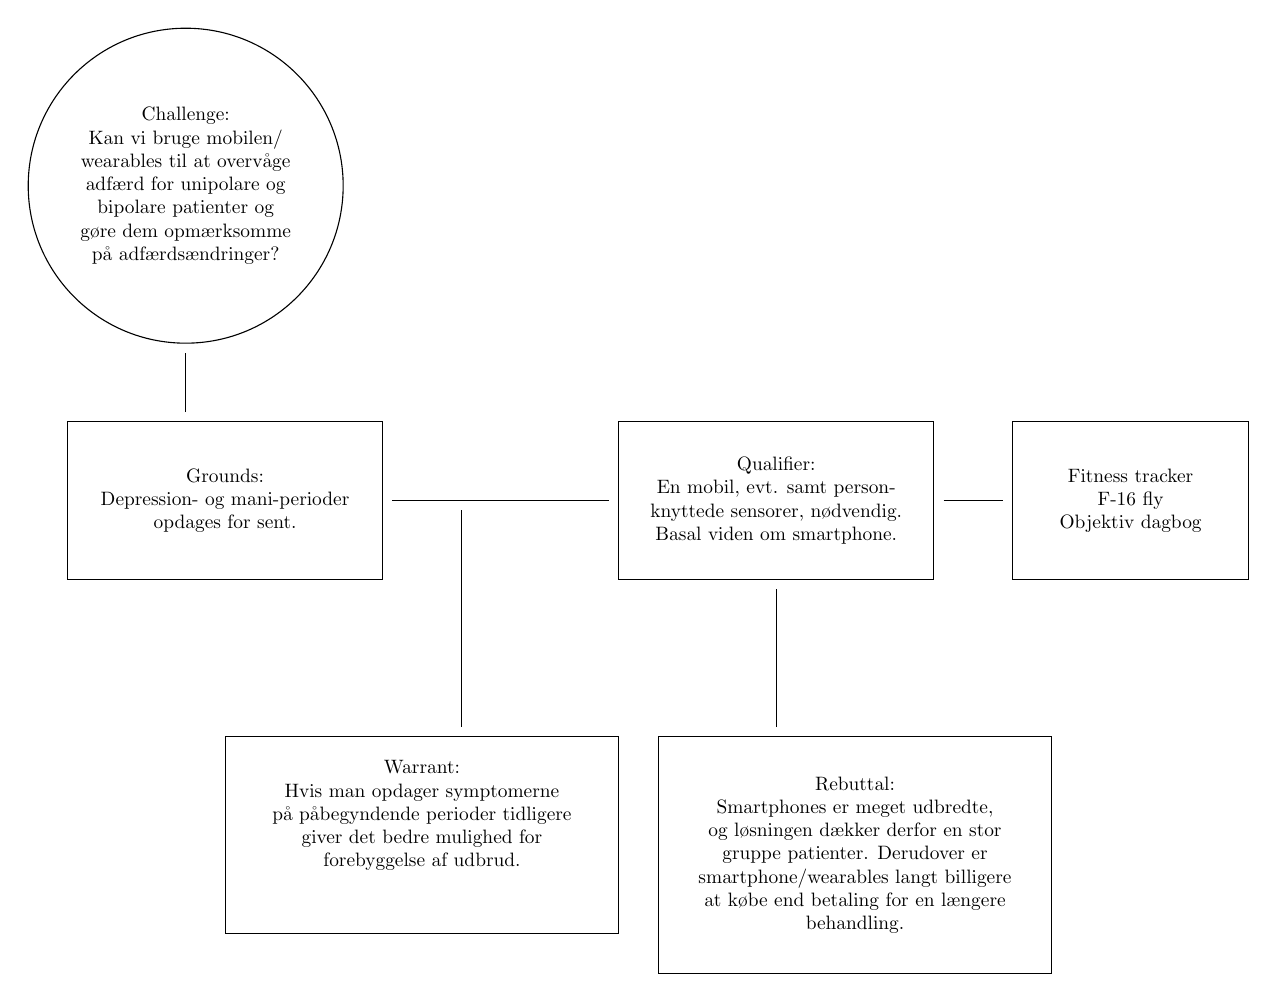
\begin{tikzpicture}

\draw  (-14,7) rectangle (-10,5);
\draw  (-12,3) rectangle (-7,0.5);
\draw  (-6.5,3) rectangle (-1.5,0);
\draw  (-7,7) rectangle (-3,5);
\draw  (-2,7) rectangle (1,5);

\node (v1) at (-10,6) {};

\node (v2) at (-7,6) {};
\draw  (v1) edge (v2);


\node (v3) at (-9,6) {};
\node (v4) at (-9,3) {};
\draw  (v3) edge (v4);
\node (v5) at (-5,3) {};
\node (v6) at (-5,5) {};
\draw  (v5) edge (v6);
\node (v7) at (-3,6) {};
\node (v8) at (-2,6) {};
\draw  (v7) edge (v8);



\draw  (-12.5,10) ellipse (2 and 2);
\node[align=center,scale=0.7] at (-12.5,10) {Challenge: \\Kan vi bruge mobilen/\\wearables  til at overvåge \\ adfærd for unipolare og \\ bipolare patienter og \\gøre dem opmærksomme\\ på adfærdsændringer?};

\node[align=center,scale=0.7] at (-12,6) {Grounds:\\Depression- og mani-perioder\\ opdages for sent.};
\node[align=center,scale=0.7] at (-9.5,2) {Warrant: \\Hvis man opdager symptomerne\\ på påbegyndende perioder tidligere\\ giver det bedre mulighed for\\ forebyggelse af udbrud.};

\node[align=center,scale=0.7] at (-5,6) {Qualifier:\\En mobil, evt. samt person-\\knyttede sensorer, nødvendig.\\ Basal viden om smartphone.};
\node[align=center,scale=0.7] at (-4,1.5) {Rebuttal:\\Smartphones er meget udbredte,\\ og løsningen dækker derfor en stor\\ gruppe patienter. Derudover er\\ smartphone/wearables langt billigere\\ at købe end betaling for en længere\\ behandling.};
\node[align=center,scale=0.7] at (-0.5,6) {Fitness tracker\\F-16 fly\\Objektiv dagbog};

\node (v10) at (-12.5,8) {};
\node (v9) at (-12.5,7) {};
\draw  (v9) edge (v10);
\end{tikzpicture}
    
    }
	\caption{Vision mønstret for projektet.}
	\label{fig:visionpattern}
\end{figure}
